\chapter{Năng lượng và hàm Hamilton}

\lectureoverview{Trước hết, ta làm rõ hơn ý nghĩa của một đối xứng tác động và ôn lại cách các phép tịnh tiến và phép quay sinh ra động lượng và mômen động lượng. Định luật bảo toàn còn thiếu là năng lượng. Đối xứng của nó là phép tịnh tiến theo thời gian, và đại lượng bảo toàn của nó là hàm Hamilton \(H=\sum_i p_i\dot q_i-L\). Phép suy ra này cũng cho thấy chính xác sự phụ thuộc thời gian tường minh truyền năng lượng như thế nào giữa một hệ con được chọn và môi trường của nó.}

\section{Các câu hỏi trước khi vào lập luận hình thức}

Chúng ta đang tiến đến mức tối thiểu tuyệt đối của cơ học cổ điển cần cho các chủ đề tiếp theo, dù vẫn còn rất nhiều nội dung cơ học đáng để học. Hai câu hỏi đã được nêu ra trước khi lập luận chính bắt đầu.

\begin{classroomqa} \audiencequestion{Sau học phần nhập môn này, những cuốn sách nào hữu ích? \lecturetimestamp{00:00:36--00:02:13}} \lecturerresponse{Tài liệu tham khảo nâng cao đã được thừa nhận là cuốn \emph{Classical Mechanics} của Herbert Goldstein. Cuốn sách của Cornelius Lanczos về các nguyên lý biến phân của cơ học là một nguồn liên quan khác. Một danh mục tài liệu đọc của lớp học hữu ích hơn việc giả vờ rằng một giảng viên có thể bao quát mọi văn bản hiện có.} \end{classroomqa}

Câu hỏi thứ hai ghi lại một thời điểm trong lịch sử của một phép đo chưa được giải quyết. Vào 2011, thí nghiệm OPERA đã báo cáo sự đến sớm biểu kiến của các neutrino được gửi từ CERN tới Gran Sasso. Độ sai lệch được báo cáo ngắn hơn xung proton dùng để tạo ra các neutrino, nên phân tích thời gian phụ thuộc vào việc so sánh các dạng xung hơn là đánh dấu một neutrino lúc phát ra rồi nhận ra chính hạt đó khi phát hiện.

\begin{classroomqa} \audiencequestion{Kết quả neutrino dường như nhanh hơn ánh sáng đã được làm sáng tỏ chưa? \lecturetimestamp{00:02:30--00:09:03}} \lecturerresponse{Khi đó chưa thể coi bất kỳ kết luận nào là có cơ sở. Dạng xung của chùm, sự nung nóng bia, và sự đồng bộ đều đòi hỏi xem xét kỹ thuật. Một đề xuất mang tính suy đoán đã xét chuyển động của một vệ tinh GPS: trong hệ quy chiếu của vệ tinh, nguồn và đầu dò chuyển động trong khi các tín hiệu định thời truyền đi, tạo ra những hiệu chỉnh cỡ vài chục nano giây. Ước lượng này thú vị như một bài tập về bậc độ lớn, nhưng nó không được nêu ra như một chẩn đoán đáng tin cậy cho thí nghiệm. Co Lorentz thông thường ở tốc độ liên quan quá nhỏ để tạo ra hiệu ứng được báo cáo. Phản ứng thích đáng là chờ phân tích thực nghiệm.} \end{classroomqa}

\begin{figure}[htbp] \centering
  \includegraphics[width=0.78\textwidth]{lecture_05_figure_07.png} \caption{Phác thảo định thời trong hệ quy chiếu vệ tinh được thảo luận trong câu hỏi lịch sử về phép đo neutrino.} \lectureframe{00:06:30} \end{figure}

Dẫu vậy, cuộc thảo luận về định thời không cần cho phần cơ học bên dưới. Tuy nhiên, nó hữu ích như một lời nhắc rằng một ước lượng quy mô có vẻ hợp lý không đồng nghĩa với một lời giải thích thực nghiệm đã được xác lập.

\section{Đối xứng tác động và việc chọn hệ}

Hãy quay lại điểm còn bị để lại quá mơ hồ trong phần bàn luận trước: chính xác thì đối xứng là gì? Hãy xét một hạt trên một đường thẳng và chỉ dẫn \begin{equation}
  x\longrightarrow x+1.
  \label{eq:l5-shift-one}
\end{equation} Có hai cách hiểu nó. Một phép biến đổi \emph{thụ động} gán lại nhãn cho các điểm trên đường thẳng. Một điểm trước đây được gọi là \(x=0\) nay có thể được gọi là \(x'=1\), nhưng hạt không hề di chuyển. Một phép biến đổi \emph{tác động} giữ các nhãn cố định và di chuyển chính hạt đó từ \(x\) đến \(x+1\). Chỉ phép toán thứ hai mới làm thay đổi vị trí của nó so với một thế ngoài.

\begin{figure}[htbp] \centering
  \includegraphics[width=0.82\textwidth]{lecture_05_figure_08.png} \caption{Quy tắc \(x\mapsto x+1\), trục tọa độ cố định và một thế ngoài phân biệt chuyển động tác động với việc gán nhãn lại thụ động.} \lectureframe{00:11:20} \end{figure}

\begin{classroomqa} \audiencequestion{Nếu việc di chuyển hạt làm thay đổi thế năng của nó, thì nguồn tạo ra thế đó có đang bị loại ra khỏi hệ không? \lecturetimestamp{00:12:19--00:14:18}} \lecturerresponse{Chính xác. Việc gọi hệ là ``một hạt trong một thế'' chia thế giới thành hạt và một môi trường có khối lượng lớn, chẳng hạn Trái Đất, tạo ra \(V(x)\). Trái Đất quả có giật lùi, nhưng khối lượng khổng lồ của nó làm cho sự giật lùi ấy có thể bỏ qua trong gần đúng này. Di chuyển hạt tương đối so với Trái Đất cố định có thể làm thay đổi \(V\); còn tịnh tiến cả hạt lẫn Trái Đất cùng nhau thì không.} \end{classroomqa}

\begin{classroomqa} \audiencequestion{Trong ví dụ phép quay trước đó, các vận tốc có thay đổi cũng như các vị trí không? \lecturetimestamp{00:14:26--00:15:29}} \lecturerresponse{Có. Một phép quay cứng theo nghĩa tác động tác dụng lên toàn bộ lịch sử, chứ không chỉ lên một vị trí tức thời đơn lẻ. Cả vị trí lẫn các vectơ vận tốc đều bị quay. Ngược lại, một phép tịnh tiến không đổi áp dụng ở mọi thời điểm làm thay đổi \(x\) nhưng để \(\dot x\) không đổi.} \end{classroomqa}

Sự phân biệt giữa hệ và môi trường sẽ còn quay lại hai lần: khi một thiết bị phụ thuộc thời gian trao đổi năng lượng với một hệ con, và khi ma sát vĩ mô che giấu năng lượng trong chuyển động vi mô không quan sát được.

\section{Các chuyển động vô cùng nhỏ trong không gian cấu hình}

Một cấu hình của một hệ cơ học tổng quát là một điểm trong không gian của các tọa độ suy rộng \(q_i\). Một phép biến đổi vô cùng nhỏ tác động dịch chuyển mọi cấu hình khả dĩ tới một cấu hình lân cận. Ta viết \begin{equation}
  \delta q_i=\epsilon f_i(q),
  \label{eq:l5-general-transformation}
\end{equation} trong đó các hàm \(f_i\) xác định một trường dịch chuyển cố định trên không gian cấu hình. Chúng có thể phụ thuộc vào mọi tọa độ và một số có thể triệt tiêu. Thừa số chung \(\epsilon\) là nhỏ; nó tách độ lớn của bước khỏi dạng của phép biến đổi.

\begin{figure}[htbp] \centering
  \includegraphics[width=0.75\textwidth]{lecture_05_figure_09.png} \caption{Một vectơ dịch chuyển gắn với mỗi điểm của không gian cấu hình.} \lectureframe{00:16:50} \end{figure}

\begin{figure}[htbp] \centering
  \includegraphics[width=0.80\textwidth]{lecture_05_figure_10.png} \caption{Phép biến đổi vô cùng nhỏ phụ thuộc tọa độ \(\delta q_i=\epsilon f_i(q)\).} \lectureframe{00:18:00} \end{figure}

Bản thân quy tắc không có sự phụ thuộc thời gian tường minh. Vì vậy, tác dụng của nó lên các vận tốc là \begin{equation}
  \delta\dot q_i=\frac{d}{dt}(\delta q_i)
  =\epsilon\sum_j\frac{\partial f_i}{\partial q_j}\dot q_j.
  \label{eq:l5-velocity-variation}
\end{equation} Đối với một phép tịnh tiến, \(f_x=1\), nên \(\delta\dot x=0\). Đối với một phép quay, \(f_i\) phụ thuộc vào vị trí, và vận tốc thay đổi.

\begin{classroomqa} \audiencequestion{Thừa số nhỏ cuối cùng trong \(\delta q_i=\epsilon f_i(q)\) có phải là cùng một hằng số tại mọi điểm không? \lecturetimestamp{00:19:58--00:20:51}} \lecturerresponse{Đúng. Hằng số duy nhất \(\epsilon\) chỉ là một công cụ để theo dõi, giúp mọi biến đổi tọa độ đều là bậc nhất theo cùng một đại lượng nhỏ. Chính các hàm \(f_i(q)\), chứ không phải \(\epsilon\), mới chứa sự phụ thuộc không gian và bản thân chúng không cần phải nhỏ.} \end{classroomqa}

\section{Điều gì làm cho phép biến đổi trở thành một đối xứng?}

Một phép biến đổi tác động nói chung làm thay đổi thế năng. Nó cũng có thể làm thay đổi động năng. Trong các tọa độ cong tuyến, hạng động năng có dạng \begin{equation}
  T=\frac12\sum_{i,j}g_{ij}(q)\dot q_i\dot q_j,
  \label{eq:l5-kinetic-metric}
\end{equation} nên việc di chuyển trong không gian cấu hình có thể làm thay đổi các hệ số của nó. Hạng quen thuộc \(r^2\dot\theta^2\) trong tọa độ cực là ví dụ đơn giản nhất.

Ở đây, một phép biến đổi là đối xứng khi \emph{toàn bộ} Lagrangian không có biến thiên bậc nhất, \begin{equation}
  \delta L=O(\epsilon^2),
  \label{eq:l5-symmetry-condition}
\end{equation} và điều này phải đúng tại mọi điểm của không gian cấu hình, không chỉ tại cấu hình do một nghiệm riêng nào đó chiếm.

Ví dụ, dưới phép biến đổi \(x\mapsto x+\epsilon\), \begin{equation}
  \delta V=\frac{\partial V}{\partial x}\epsilon.
  \label{eq:l5-potential-variation}
\end{equation} Nếu biểu thức này triệt tiêu với mọi \(x\) khả dĩ, thì \(\partial V/\partial x=0\): thế không phụ thuộc vào \(x\). Nếu nó không đổi dưới các phép tịnh tiến theo mọi hướng trong không gian, thì nó là hằng số.

\begin{figure}[htbp] \centering
  \includegraphics[width=0.80\textwidth]{lecture_05_figure_11.png} \caption{Một phép tịnh tiến theo \(x\) được kiểm tra đối với một thế \(V(y)\) không phụ thuộc vào \(x\).} \lectureframe{00:23:40} \end{figure}

Đối với một họ trơn một tham số, việc biến thiên bậc nhất triệt tiêu tại mọi điểm cho phép ta hợp thành các bước vô cùng nhỏ thành một đối xứng hữu hạn.

\begin{classroomqa} \audiencequestion{Động năng và thế năng có phải bất biến riêng rẽ không? \lecturetimestamp{00:24:44--00:25:33}} \lecturerresponse{Không. Chỉ tổng Lagrangian phải bất biến. Một số Lagrangian chứa các hạng trộn tọa độ--vận tốc và không cho phép một sự tách hữu ích thành \(T\) và \(V\), nên tính bất biến riêng rẽ thậm chí có thể không phải là một câu hỏi có ý nghĩa.} \end{classroomqa}

\begin{classroomqa} \audiencequestion{Liệu ``không đổi'' có nghĩa là hoàn toàn không đổi, hay chỉ là thay đổi đủ nhỏ để bỏ qua? \lecturetimestamp{00:25:34--00:28:59}} \lecturerresponse{Đối với một phép biến đổi vô cùng nhỏ, điều đó có nghĩa là không có hạng nào tỉ lệ với \(\epsilon\). Các hạng bậc \(\epsilon^2\) bị bỏ qua trong phép tính cục bộ. Vì điều kiện bậc nhất giữ đúng ở khắp nơi dọc theo quỹ đạo một tham số, việc lặp lại bước cục bộ cho ta tính bất biến hữu hạn.} \end{classroomqa}

\section{Khôi phục động lượng và mômen động lượng}

Đối với các đối xứng điểm chính xác, không phụ thuộc thời gian được xét ở đây, kết quả đã chứng minh trước đó là \begin{equation}
  Q=\sum_i p_i f_i(q),
  \qquad
  p_i=\frac{\partial L}{\partial\dot q_i},
  \qquad
  \dot Q=0.
  \label{eq:l5-noether-charge}
\end{equation} Thừa số \(\epsilon\) không thuộc về \(Q\); nó chỉ đo xem ta đi xa đến đâu dọc theo quỹ đạo đối xứng.

\begin{figure}[htbp] \centering
  \includegraphics[width=0.82\textwidth]{lecture_05_figure_12.png} \caption{Độ dịch chuyển vô cùng nhỏ tổng quát và điện tích Noether bảo toàn của nó.} \lectureframe{00:30:00} \end{figure}

Đối với một phép tịnh tiến theo \(x\), \(f_x=1\), và \(Q=p_x\). Bất biến tịnh tiến đầy đủ cho bảo toàn cả ba thành phần của động lượng. Với nhiều hạt tương tác, đối xứng này tịnh tiến mọi hạt cùng nhau, nên \begin{equation}
  \mathbf P=\sum_a\mathbf p_a
  \label{eq:l5-total-momentum}
\end{equation} được bảo toàn khi các tương tác chỉ phụ thuộc vào các vị trí tương đối. Di chuyển một hạt tương đối so với phần còn lại không phải là đối xứng đó.

\begin{figure}[htbp] \centering
  \includegraphics[width=0.80\textwidth]{lecture_05_figure_13.png} \caption{Một phép tịnh tiến chung dẫn đến bảo toàn tổng động lượng, theo từng thành phần.} \lectureframe{00:32:50} \end{figure}

Đối với một phép quay vô cùng nhỏ trong mặt phẳng \(x\)-\(y\), hãy chọn quy ước định hướng \begin{equation}
  \delta x=-y\epsilon,
  \qquad
  \delta y=x\epsilon.
  \label{eq:l5-planar-rotation}
\end{equation} Nó bảo toàn bán kính vì \begin{equation}
  \delta(x^2+y^2)
  =2x\delta x+2y\delta y=0.
  \label{eq:l5-radius-invariance}
\end{equation}

\begin{figure}[htbp] \centering
  \includegraphics[width=0.76\textwidth]{lecture_05_figure_14.png} \caption{Hình học và công thức tọa độ cho một phép quay phẳng vô cùng nhỏ.} \lectureframe{00:35:05} \end{figure}

Lấy đạo hàm theo thời gian của phương trình~\eqref{eq:l5-planar-rotation} cũng làm quay các vận tốc. Do đó \(\dot x^2+\dot y^2\) là bất biến, và một thế tâm \(V(\sqrt{x^2+y^2})\) làm cho toàn bộ Lagrangian không đổi. Điện tích là \begin{equation}
  Q=-yp_x+xp_y=(\mathbf r\times\mathbf p)_z.
  \label{eq:l5-angular-charge}
\end{equation}

\begin{figure}[htbp] \centering
  \includegraphics[width=0.76\textwidth]{lecture_05_figure_15.png} \caption{Điện tích Noether của phép quay, tức thành phần \(z\) của mômen động lượng.} \lectureframe{00:38:50} \end{figure}

Các phép quay trong những mặt phẳng tọa độ khác cho các thành phần còn lại. Với nhiều hạt, vectơ bảo toàn là \begin{equation}
  \mathbf J=\sum_a\mathbf r_a\times\mathbf p_a.
  \label{eq:l5-total-angular-momentum}
\end{equation} Một hành tinh trong một thế tâm của sao là ví dụ cơ bản: bất biến dưới mọi phép quay suy ra bảo toàn mọi thành phần của mômen động lượng.

\begin{classroomqa} \audiencequestion{Điều gì xảy ra tại một điểm nhọn sắc, nơi đạo hàm từ một phía khác với đạo hàm từ phía kia? \lecturetimestamp{00:42:25--00:44:21}} \lecturerresponse{Đó là một sự dè dặt chính đáng. Lập luận hiện tại giả thiết các hàm khả vi với đạo hàm duy nhất. Một cân bằng không bền, chẳng hạn một vật được giữ thăng bằng tại một cực đại trơn, tự nó không phải là vấn đề: đạo hàm ở đó tồn tại và triệt tiêu. Một điểm nhọn thực sự đòi hỏi một cách xử lý đã sửa đổi.} \end{classroomqa}

\begin{classroomqa} \audiencequestion{Nếu tham số biến đổi không phụ thuộc thời gian, tại sao một phép quay lại làm thay đổi các vận tốc? \lecturetimestamp{00:44:23--00:45:23}} \lecturerresponse{Tham số là hằng số, nhưng trường dịch chuyển thì phụ thuộc tọa độ. Quy tắc phổ quát là \(\delta\dot q_i=d(\delta q_i)/dt\). Một phép tịnh tiến có \(\delta x\) hằng, còn một phép quay có \(\delta x=-y\epsilon\) và do đó \(\delta\dot x=-\dot y\epsilon\).} \end{classroomqa}

\section{Vượt ra ngoài dạng sơ cấp động năng trừ thế năng}

Trong tọa độ Descartes đối với các hạt phi tương đối thông thường không có từ trường, \(L=T-V\). Các tọa độ tổng quát hơn cho dạng toàn phương của phương trình~\eqref{eq:l5-kinetic-metric}. Từ trường đưa vào một hạng tuyến tính theo vận tốc, có dạng sơ đồ \(\mathbf A(q)\cdot\dot{\mathbf q}\), trộn lẫn tọa độ và vận tốc. Trong trường hợp như vậy, tốt hơn nên coi \(L(q,\dot q,t)\) là một hàm duy nhất hơn là ép mọi hạng vào các ngăn động năng và thế năng theo quy ước.

\begin{figure}[htbp] \centering
  \includegraphics[width=0.80\textwidth]{lecture_05_figure_16.png} \caption{Một hạng động năng toàn phương tổng quát phụ thuộc tọa độ bên cạnh một thế chỉ phụ thuộc tọa độ.} \lectureframe{00:47:20} \end{figure}

\begin{classroomqa}
  \audiencequestion{Vì sao một Lagrangian có thể không tách gọn được thành động năng và thế năng, và khi đó nó còn được định nghĩa là \(T-V\) không?
  \lecturetimestamp{00:45:26--00:48:13}}
  \lecturerresponse{Trở ngại có thể đến từ các tọa độ cong, hoặc từ những tương tác thật sự phụ thuộc vào vận tốc như từ tính. Chỉ khi Lagrangian gồm một dạng bậc hai theo vận tốc trừ đi một hàm chỉ phụ thuộc tọa độ thì ta mới gọi các phần ấy là \(T\) và \(V\). Nếu không, Lagrangian vẫn hoàn toàn là một hàm hợp lệ của \(q\) và \(\dot q\), nhưng phép tách ấy không còn hữu ích. Định nghĩa tổng quát đúng của năng lượng sẽ xuất phát từ Hamiltonian.}
\end{classroomqa}

\begin{classroomqa}
  \audiencequestion{Ví dụ dây xích treo ở buổi đầu tiên có phải là một ứng dụng của nguyên lý tác dụng tối thiểu không?
  \lecturetimestamp{00:48:15--00:49:45}}
  \lecturerresponse{Đó là một bài toán cân bằng được chi phối bởi năng lượng tối thiểu, chứ không phải một lịch sử được chọn bởi tác dụng dừng. Đối với một nghiệm tĩnh của một hệ \(T-V\) thông thường, \(\dot p_i=0\) và phương trình Euler--Lagrange rút gọn thành \(\partial V/\partial q_i=0\), là điều kiện cho một điểm dừng của thế năng.}
\end{classroomqa}

Động lượng và mômen động lượng giờ đây đã được gắn với các đối xứng không gian. Đại lượng còn thiếu một cách nổi bật là năng lượng.

\section{Tính bất biến dưới phép tịnh tiến theo thời gian}

Hãy hình dung một thí nghiệm bắt đầu tại \(t_0\), kết thúc tại \(t_1\), và cho ra một kết quả. Lặp lại đúng sự chuẩn bị ấy muộn hơn, bắt đầu tại \(t_0+\Delta t\) và kết thúc tại \(t_1+\Delta t\). Nếu kết quả không đổi, thì hệ bất biến dưới một phép tịnh tiến chủ động theo thời gian.

\begin{figure}[htbp]
  \centering
  \includegraphics[width=0.82\textwidth]{lecture_05_figure_17.png}
  \caption{Một thí nghiệm và bản sao của nó được tịnh tiến theo thời gian trong lịch sử không gian cấu hình.}
  \lectureframe{00:52:45}
\end{figure}

Một hạt tích điện giữa các bản tụ minh họa sự thất bại của đối xứng này. Khi điện tích trên bản được giữ cố định, có thể thực hiện cùng một thí nghiệm vào bất kỳ thời điểm nào. Nếu một máy phát bên ngoài đang nạp đều các bản tụ, hạt sẽ thấy một điện trường khác nhau tùy theo lúc nó được thả ra. Khi đó hạt là một phân hệ được dẫn động tường minh.

\begin{figure}[htbp]
  \centering
  \includegraphics[width=0.82\textwidth]{lecture_05_figure_18.png}
  \caption{Các bản tụ cố định và các bản tụ biến đổi từ bên ngoài được đối chiếu bên cạnh sơ đồ tịnh tiến theo thời gian.}
  \lectureframe{00:54:45}
\end{figure}

Điểm ấy cũng xuất hiện ở một dao động tử,
\begin{equation}
  L=\frac12m\dot x^2-\frac12k(t)x^2.
  \label{eq:l5-driven-oscillator}
\end{equation}
Một điện trường hay từ trường ngoài có thể từ từ làm biến đổi vật liệu và vì thế làm thay đổi hằng số đàn hồi hiệu dụng của nó. Nếu \(k\) biến thiên, việc tịnh tiến thí nghiệm dao động tử theo thời gian sẽ làm thay đổi kết quả.

\begin{figure}[htbp]
  \centering
  \includegraphics[width=0.78\textwidth]{lecture_05_figure_19.png}
  \caption{Các hạng động năng và thế năng của dao động tử trong phần thảo luận về một hằng số đàn hồi phụ thuộc thời gian.}
  \lectureframe{00:56:45}
\end{figure}

Nếu thiết bị làm thay đổi \(k\) được gộp vào trong hệ, thì toàn bộ thí nghiệm kín lại có thể được tịnh tiến theo thời gian và toàn bộ năng lượng của nó được bảo toàn. Sự không bảo toàn có vẻ bề ngoài ấy là sự trao đổi năng lượng qua một biên do ta chọn.

Trong giờ nghỉ, tham số biến đổi nhỏ được đổi tên thành \(\epsilon\), để tránh biểu thức gây rối mắt \(\delta x=\delta\). Một đề xuất trên lớp về một cuốn sách viết về Emmy Noether cũng được ghi vào danh sách đọc chung.

\begin{classroomqa}
  \audiencequestion{Nếu Lagrangian không được cho dưới dạng \(T-V\), thì nó từ đâu ra?
  \lecturetimestamp{01:00:17--01:02:24}}
  \lecturerresponse{Nó có thể được suy ra từ thực nghiệm, được tái dựng từ các phương trình chuyển động đã biết, được phỏng đoán từ đối xứng và các nguyên lý lý thuyết khác, hoặc được tìm ra bằng thử và sai. Một khi \(L(q,\dot q,t)\) đã được cho, phép tính Euler--Lagrange sẽ biến nó thành các phương trình chuyển động. Lập luận hình thức không đòi hỏi ta phải giải quyết trước nguồn gốc của nó.}
\end{classroomqa}

Tiêu chuẩn thao tác để kiểm tra tính bất biến tịnh tiến theo thời gian giờ đây là trực tiếp. Nếu biết \(q\) và \(\dot q\) là đủ để xác định \(L\), mà không cần biết thêm thời gian trên đồng hồ, thì
\begin{equation}
  \frac{\partial L}{\partial t}=0.
  \label{eq:l5-no-explicit-time}
\end{equation}
Điều này không nói rằng \(L(q(t),\dot q(t))\) là hằng dọc theo một chuyển động. Nó chỉ nói rằng không có sự phụ thuộc thời gian nào ngoài sự phụ thuộc do các tọa độ và vận tốc đang biến thiên mang theo.

Một ví dụ bị dẫn động khác là một tạ đôi nặng đang quay. Nếu chuyển động được ấn định trước của nó tạo ra một thế hấp dẫn biến thiên theo thời gian cho một hạt thử nhẹ, thì Lagrangian của hạt thử phụ thuộc tường minh vào thời gian. Ngược lại, nếu xử lý tạ đôi một cách động lực học, thì ta mở rộng hệ và loại bỏ sự phụ thuộc thời gian bên ngoài đó.

\begin{figure}[htbp]
  \centering
  \includegraphics[width=0.80\textwidth]{lecture_05_figure_20.png}
  \caption{Một tạ đôi quay được ấn định trước đóng vai trò như một nguồn ngoài phụ thuộc thời gian đối với một hạt nhẹ hơn.}
  \lectureframe{01:06:25}
\end{figure}

\section{Suy ra Hamiltonian}

Giả sử ta chưa biết công thức của năng lượng và đoán rằng có lẽ chính Lagrangian được bảo toàn. Phép kiểm tra trực tiếp là lấy đạo hàm của nó dọc theo một quỹ đạo thực sự. Trước hết, cho đơn giản, hãy xét trường hợp không có sự phụ thuộc thời gian tường minh:
\begin{equation}
  \frac{dL}{dt}
  =\sum_i\left(
    \frac{\partial L}{\partial q_i}\dot q_i
    +\frac{\partial L}{\partial\dot q_i}\ddot q_i
  \right).
  \label{eq:l5-chain-rule-no-time}
\end{equation}

\begin{figure}[htbp]
  \centering
  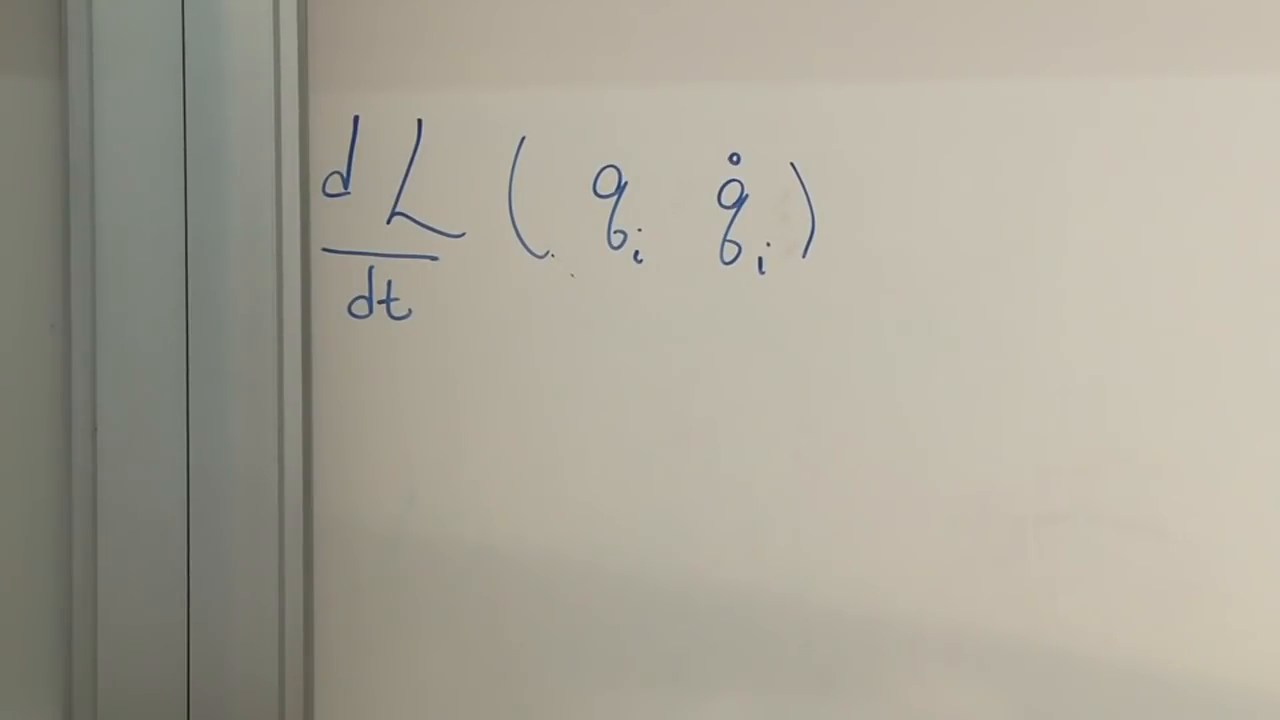
\includegraphics[width=0.72\textwidth]{lecture_05_figure_02.png}
  \caption{Bắt đầu lấy đạo hàm của \(L(q_i,\dot q_i)\) dọc theo quỹ đạo.}
  \lectureframe{01:08:51}
\end{figure}

\begin{classroomqa}
  \audiencequestion{Có thiếu một phép lấy tổng trong biểu thức quy tắc dây chuyền không?
  \lecturetimestamp{01:10:39--01:11:05}}
  \lecturerresponse{Có. Mỗi tọa độ và mỗi vận tốc đều có thể làm thay đổi Lagrangian, nên cả hai hạng đều được lấy tổng theo \(i\).}
\end{classroomqa}

Dùng xung lượng chính tắc và phương trình Euler--Lagrange,
\begin{equation}
  p_i=\frac{\partial L}{\partial\dot q_i},
  \qquad
  \dot p_i=\frac{\partial L}{\partial q_i}.
  \label{eq:l5-p-and-pdot}
\end{equation}
Khi đó phương trình ~\eqref{eq:l5-chain-rule-no-time} trở thành
\begin{align}
  \frac{dL}{dt}
  &=\sum_i(\dot p_i\dot q_i+p_i\ddot q_i)
  \notag\\
  &=\frac{d}{dt}\sum_i p_i\dot q_i.
  \label{eq:l5-product-rule}
\end{align}
Cái ``phép màu'' ấy thực ra chỉ là quy tắc tích.

\begin{figure}[htbp]
  \centering
  \includegraphics[width=0.84\textwidth]{lecture_05_figure_21.png}
  \caption{Quy tắc dây chuyền được biến đổi, dùng các phương trình chuyển động, thành đạo hàm của \(\sum_i p_i\dot q_i\).}
  \lectureframe{01:13:45}
\end{figure}

\begin{classroomqa}
  \audiencequestion{Ở \(q_i\) cuối cùng trong tích có nên đặt một chấm hay hai chấm không?
  \lecturetimestamp{01:14:31--01:15:32}}
  \lecturerresponse{Trong tích đó là \(p_i\dot q_i\), với một chấm. Lấy đạo hàm tích cho
  \(\dot p_i\dot q_i+p_i\ddot q_i\), điều này giải thích hai chấm ở hạng thứ hai khi khai triển.}
\end{classroomqa}

Lấy hiệu hai đạo hàm ấy cho một tổ hợp được bảo toàn. Theo quy ước lịch sử, người ta chọn số đối của nó và gọi đó là Hamiltonian:
\begin{equation}
  H=\sum_i p_i\dot q_i-L.
  \label{eq:l5-hamiltonian-definition}
\end{equation}

\begin{figure}[htbp]
  \centering
  \includegraphics[width=0.80\textwidth]{lecture_05_figure_22.png}
  \caption{Tổ hợp được bảo toàn \(L-\sum_i p_i\dot q_i=-H\) và định nghĩa Hamiltonian.}
  \lectureframe{01:18:05}
\end{figure}

Đối với một hạt trong một thế,
\begin{equation}
  L=\frac12m\dot x^2-V(x),
  \qquad p=m\dot x.
  \label{eq:l5-particle-lagrangian}
\end{equation}
Vì vậy
\begin{align}
  H&=p\dot x-L
  \notag\\
   &=m\dot x^2-\left(\frac12m\dot x^2-V(x)\right)
  \notag\\
   &=\frac12m\dot x^2+V(x)=T+V.
  \label{eq:l5-particle-energy}
\end{align}

\begin{figure}[htbp]
  \centering
  \includegraphics[width=0.86\textwidth]{lecture_05_figure_23.png}
  \caption{Hamiltonian của một hạt trong một thế rút về động năng cộng thế năng quen thuộc.}
  \lectureframe{01:20:50}
\end{figure}

Phép suy ra này không giả sử một dạng cụ thể nào của \(L\). Vì vậy phương trình ~\eqref{eq:l5-hamiltonian-definition}, chứ không phải \(T+V\), mới là định nghĩa tổng quát của năng lượng trong hình thức này.

\section{Sự phụ thuộc thời gian tường minh và trao đổi năng lượng}

Khôi phục sự phụ thuộc thời gian tường minh trong quy tắc dây chuyền:
\begin{equation}
  \frac{dL}{dt}
  =\sum_i\left(
    \frac{\partial L}{\partial q_i}\dot q_i
    +\frac{\partial L}{\partial\dot q_i}\ddot q_i
  \right)
  +\frac{\partial L}{\partial t}.
  \label{eq:l5-full-chain-rule}
\end{equation}
Vế trái là đạo hàm toàn phần dọc theo chuyển động. Đạo hàm riêng cuối cùng giữ \(q\) và \(\dot q\) cố định và chỉ lấy đạo hàm theo các tham số biến đổi từ bên ngoài. Lặp lại đúng bước quy tắc tích ấy cho
\begin{equation}
  \boxed{\frac{dH}{dt}=-\frac{\partial L}{\partial t}}.
  \label{eq:l5-hamiltonian-time}
\end{equation}

\begin{figure}[htbp]
  \centering
  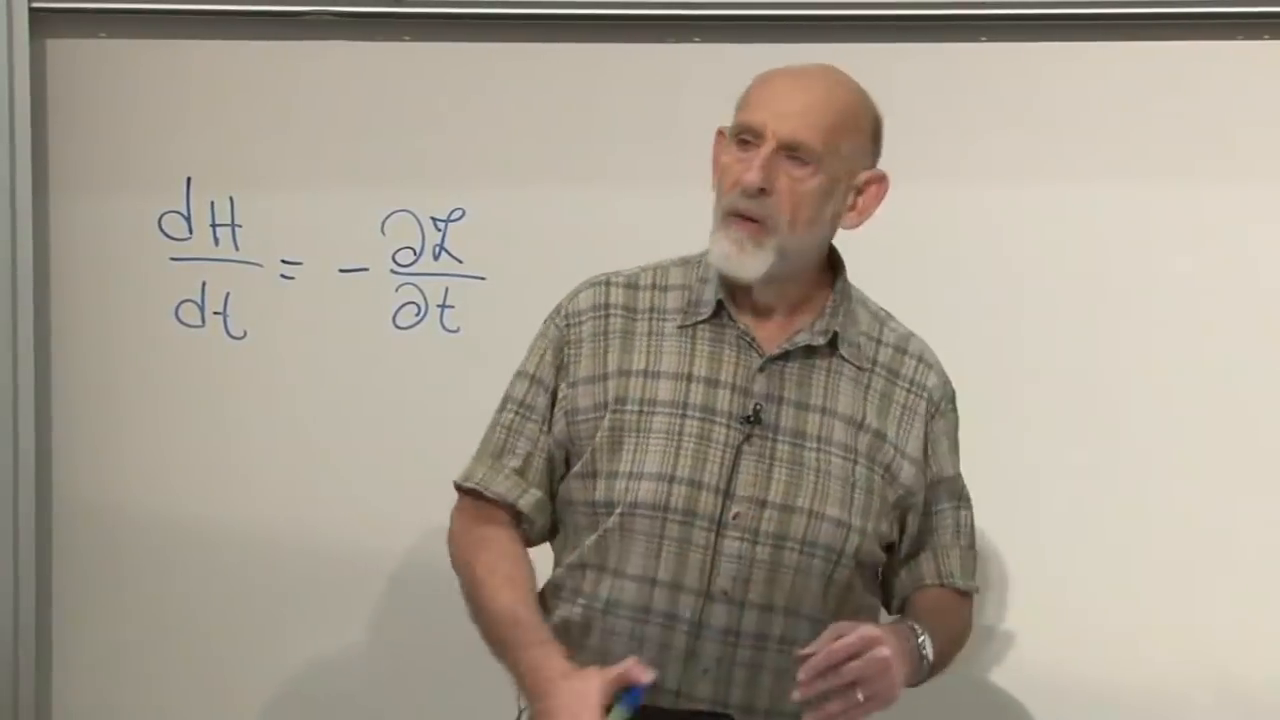
\includegraphics[width=0.70\textwidth]{lecture_05_figure_04.png}
  \caption{Hamiltonian chỉ thay đổi thông qua sự phụ thuộc thời gian tường minh của Lagrangian.}
  \lectureframe{01:37:22}
\end{figure}

Đối với dao động tử bị dẫn động trong phương trình ~\eqref{eq:l5-driven-oscillator},
\begin{equation}
  \frac{\partial L}{\partial t}
  =-\frac12\dot k(t)x^2,
  \qquad
  \dot H=\frac12\dot k(t)x^2.
  \label{eq:l5-driven-energy-rate}
\end{equation}
Tại \(x=0\), tốc độ tức thời triệt tiêu; ra xa gốc tọa độ, việc thay đổi hằng số đàn hồi thực hiện công với tốc độ tỉ lệ với \(x^2\dot k\).

\begin{classroomqa}
  \audiencequestion{Nếu năng lượng không được bảo toàn, thì định nghĩa của nó có phải là đạo hàm theo thời gian của Hamiltonian không?
  \lecturetimestamp{01:27:11--01:28:04}}
  \lecturerresponse{Không. Năng lượng là \(H\). Đạo hàm của nó cho ta biết năng lượng ấy thay đổi như thế nào. Khi Lagrangian có dạng quen thuộc, \(H=T+V\); khi không phải vậy, phương trình ~\eqref{eq:l5-hamiltonian-definition} cung cấp định nghĩa. Mở rộng hệ để bao gồm cả tác nhân dẫn động bên ngoài sẽ khôi phục sự bảo toàn của Hamiltonian toàn phần.}
\end{classroomqa}

\begin{classroomqa}
  \audiencequestion{Điều này áp dụng thế nào cho người quan sát đã nói trước đó trên một đu quay đang quay, nơi xuất hiện các hạng ly tâm và Coriolis?
  \lecturetimestamp{01:28:08--01:29:52}}
  \lecturerresponse{Một hệ tọa độ quay đều là một phép đổi biến phụ thuộc thời gian, không phải một đối xứng không gian cố định và cũng không phải một phép tịnh tiến đơn giản theo thời gian. Lagrangian đã biến đổi của nó có thể được dùng để xây dựng một Hamiltonian, nhưng phép tính riêng ấy tốt hơn nên để lại đến khi bàn về lực từ, vì phép đại số có dạng liên hệ rất gần.}
\end{classroomqa}

\section{Toàn cảnh bộ công cụ Lagrangian}

Giờ đây toàn bộ cấu trúc có thể được viết thành một khối công thức gọn:
\begin{align}
  L&=L(q_i,\dot q_i,t),
  \notag\\
  p_i&=\frac{\partial L}{\partial\dot q_i},
  \qquad
  \dot p_i=\frac{\partial L}{\partial q_i},
  \notag\\
  \delta q_i&=\epsilon f_i(q)
  \quad\Longrightarrow\quad
  Q=\sum_i p_i f_i(q),\quad \dot Q=0,
  \notag\\
  H&=\sum_i p_i\dot q_i-L,
  \qquad
  \dot H=-\frac{\partial L}{\partial t}.
  \label{eq:l5-toolkit}
\end{align}

\begin{figure}[htbp]
  \centering
  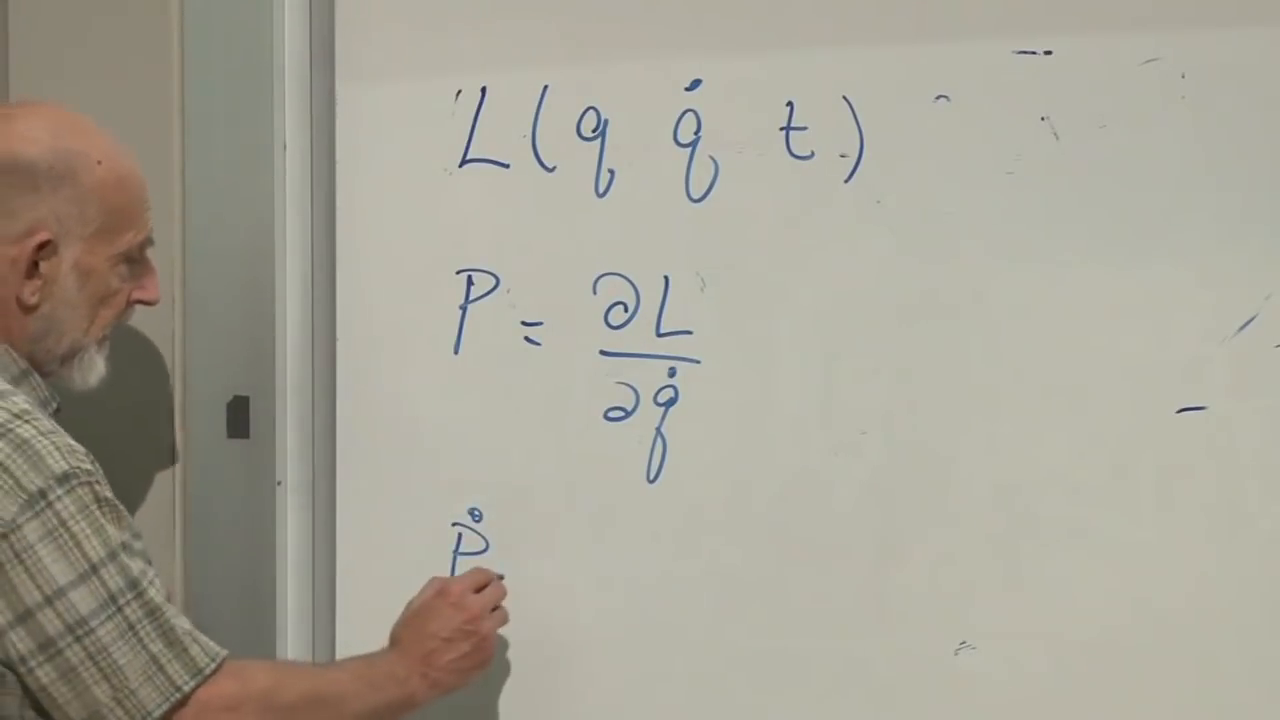
\includegraphics[width=0.66\textwidth]{lecture_05_figure_03.png}
  \caption{Phần tổng kết trên bảng bắt đầu với \(L(q,\dot q,t)\), xung lượng chính tắc và phương trình Euler--Lagrange.}
  \lectureframe{01:31:37}
\end{figure}

Những công thức này chứa một định nghĩa, các phương trình chuyển động, tích lượng của một đối xứng liên tục thông thường và tích lượng của phép tịnh tiến theo thời gian. Có rất ít mẹo; điều quan trọng là phải có khả năng tự suy ra lại chúng thay vì học thuộc những biểu thức rời rạc.

\section{Vì sao dùng cơ học Lagrange hay cơ học Hamilton?}

\begin{classroomqa}
  \audiencequestion{Có thể mô tả cơ học như nhau bằng \(L\) hoặc \(H\) không, và vì sao lại chọn một hình thức thay vì hình thức kia?
  \lecturetimestamp{01:37:16--01:39:18}}
  \lecturerresponse{Chúng tương đương khi phép biến đổi Legendre là chính quy, nhưng mỗi bên nhấn mạnh những cấu trúc khác nhau. Hình thức Lagrange khởi đầu một cách tự nhiên từ tác dụng dừng. Cơ học Hamilton lúc đầu trừu tượng hơn, nhưng các phương trình của nó đơn giản và nó trở thành trung tâm trong cơ học lượng tử. Hamiltonian là năng lượng, nhưng vai trò của nó còn lớn hơn nhiều so với chỉ riêng định luật bảo toàn.}
\end{classroomqa}

\begin{classroomqa}
  \audiencequestion{Newton có biết dạng Hamiltonian của định luật bảo toàn năng lượng không?
  \lecturetimestamp{01:39:29--01:39:56}}
  \lecturerresponse{Không phải trong cách phát biểu này, theo chừng mực tư liệu lịch sử cho thấy. Khuôn khổ mà Newton phát biểu là định luật lực \(F=ma\).}
\end{classroomqa}

\begin{classroomqa}
  \audiencequestion{Vì sao mọi hệ vật lý đều phải có một Lagrangian? Điều đó chỉ là vấn đề thực nghiệm thôi sao?
  \lecturetimestamp{01:39:57--01:42:37}}
  \lecturerresponse{Đối với các hệ kín đang được xét, đó là một sự kiện thực nghiệm và đồng thời cũng theo sau từ mô tả lượng tử sâu hơn. Người ta có thể dựng ra những phương trình vi phân nhất quán về mặt toán học mà không phải là các phương trình Euler--Lagrange. Chẳng hạn, \(\dot x=-x\) hoàn toàn giải được, nhưng với tư cách một định luật cơ bản kín cho một tọa độ duy nhất, nó mang tính chất làm mất thông tin của sự tiêu tán. Cơ học cổ điển không đi trước cơ học lượng tử về mặt logic; cấu trúc nền tảng của nó được thừa hưởng từ cơ học lượng tử. Lý do chi tiết phải để lại sau.}
\end{classroomqa}

\begin{classroomqa}
  \audiencequestion{Nếu mọi hệ kín thực sự đều có một Lagrangian, thì có phải mọi hàm mà ta gọi là Lagrangian đều tương ứng với một hệ tìm thấy trong tự nhiên không?
  \lecturetimestamp{01:42:39--01:42:54}}
  \lecturerresponse{Không. Phép tính hình thức chấp nhận nhiều hàm không được hiện thực hóa bởi bất kỳ hệ vật lý đã biết nào.}
\end{classroomqa}

\begin{classroomqa}
  \audiencequestion{Lagrangian có chủ yếu là một công cụ để nghĩ ra các thế không?
  \lecturetimestamp{01:42:54--01:43:32}}
  \lecturerresponse{Nó còn rộng hơn thế. Nó có thể dùng để tổ chức các hệ cơ học khả dĩ, và thường là con đường thực hành ngắn nhất để đi tới các phương trình chuyển động.}
\end{classroomqa}

Con lắc kép cho thấy ưu thế thực hành đó. Chọn hai góc, tính vận tốc của cả hai khối lượng theo các góc ấy và các đạo hàm theo thời gian của chúng, lập \(T-V\), rồi để các phương trình Euler--Lagrange xử lý ngầm các lực liên kết. Cách này gọn hơn đáng kể so với việc phân giải mọi lực căng và gia tốc bằng \(F=ma\).

\begin{figure}[htbp]
  \centering
  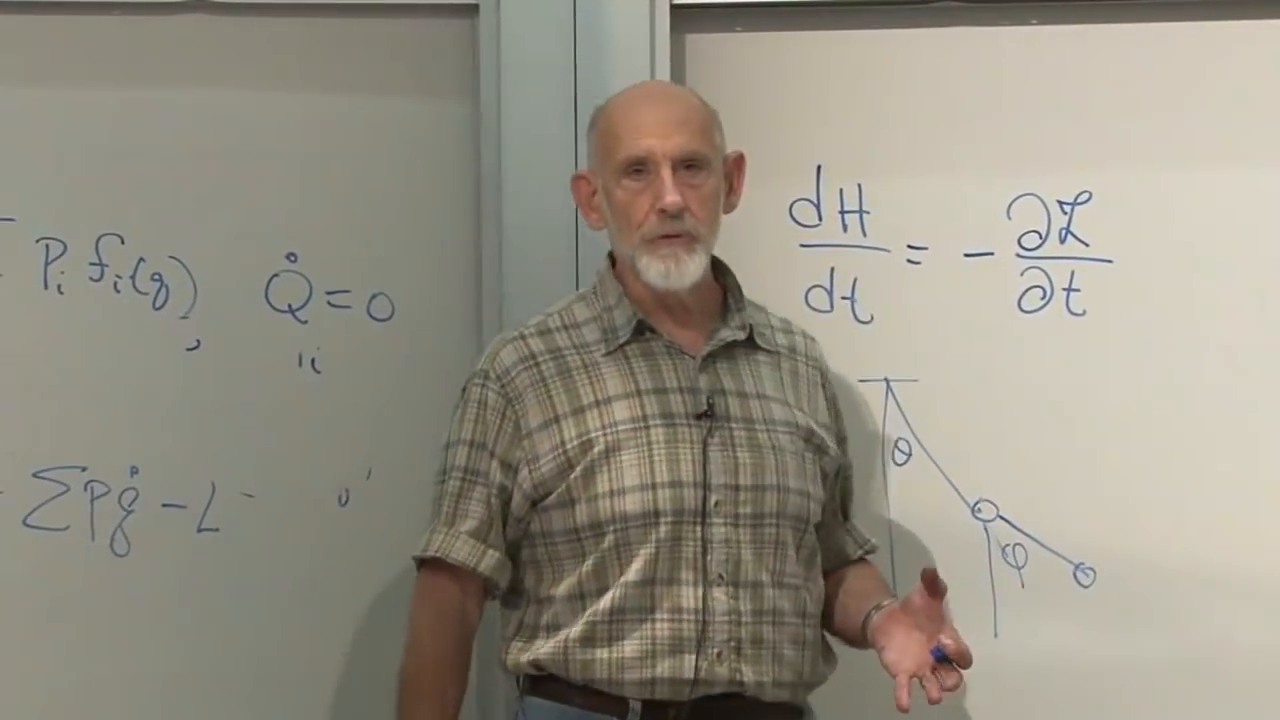
\includegraphics[width=0.84\textwidth]{lecture_05_figure_05.png}
  \caption{Đẳng thức về tốc độ biến thiên năng lượng vẫn còn trên bảng bên cạnh hình phác con lắc kép.}
  \lectureframe{01:45:39}
\end{figure}

\begin{figure}[htbp]
  \centering
  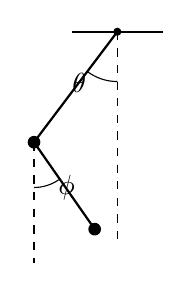
\begin{tikzpicture}[scale=1.15]
    \draw[thick] (-0.5,0) -- (0.5,0);
    \fill (0,0) circle (0.045);
    \draw[dashed] (0,0) -- (0,-2.3);
    \draw[thick] (0,0) -- (-0.92,-1.22);
    \fill (-0.92,-1.22) circle (0.07);
    \draw[dashed] (-0.92,-1.22) -- (-0.92,-2.55);
    \draw[thick] (-0.92,-1.22) -- (-0.25,-2.18);
    \fill (-0.25,-2.18) circle (0.07);
    \draw (0,-0.55) arc (-90:-127:0.55);
    \node at (-0.42,-0.56) {$\theta$};
    \draw (-0.92,-1.72) arc (-90:-55:0.48);
    \node at (-0.56,-1.72) {$\phi$};
  \end{tikzpicture}
  \caption{Các tọa độ góc suy rộng cho một con lắc kép.}
\end{figure}

Đổi biến cũng hiệu quả tương tự: biến đổi một Lagrangian rồi suy ra các phương trình của nó, thay vì biến đổi riêng rẽ từng phương trình lực.

\begin{classroomqa}
\audiencequestion{Con lắc kép về cơ bản có phải là một hệ ba vật khác, như Mặt Trời, Trái Đất và Mặt Trăng, trong đó một vật được xem như điểm tựa không?
\lecturetimestamp{01:45:06--01:45:25}}
\lecturerresponse{Phép so sánh đó nắm đúng cấu trúc phân cấp, mặc dù các thanh áp đặt những ràng buộc khác. Trong cả hai trường hợp, trong một phép gần đúng, một thành phần rất nặng hoặc cố định có thể được coi là cấu trúc quy chiếu.}
\end{classroomqa}

\begin{classroomqa}
\audiencequestion{Con lắc kép dùng \(T-V\), mặc dù ta vừa nhấn mạnh các Lagrangian tổng quát hơn. Khi nào \(T-V\) có giá trị?
\lecturetimestamp{01:46:08--01:46:58}}
\lecturerresponse{Đối với các hạt phi tương đối tính thông thường được xét trong một hệ quy chiếu quán tính, và không có sự ghép từ tính phụ thuộc vận tốc, dạng quen thuộc đó áp dụng được. Các hệ quy chiếu quay, các hệ tương đối tính và từ trường đòi hỏi những số hạng tổng quát hơn.}
\end{classroomqa}

\begin{classroomqa}
\audiencequestion{Va chạm có nằm ngoài mô tả này không?
\lecturetimestamp{01:47:00--01:48:05}}
\lecturerresponse{Va chạm đàn hồi phát sinh từ các lực tầm ngắn và do đó từ các thế năng. Va chạm không đàn hồi vẫn là cơ học ở mức vi mô, nhưng năng lượng đi vào các dao động nội, biến dạng và nhiệt. Một mô tả khối tâm bỏ qua các bậc tự do đó là không đầy đủ.}
\end{classroomqa}

\begin{classroomqa}
\audiencequestion{Một quả bóng chày bị gậy đánh trúng có thể được phân tích bằng \(F=ma\) không?
\lecturetimestamp{01:48:05--01:48:33}}
\lecturerresponse{Chỉ ở mức thô. Một mô tả đầy đủ phải theo dõi biến dạng, sự tăng nhiệt, khả năng quả bóng bị hư hại, và có lẽ cả chiếc gậy bị gãy. Chính các bậc tự do nội đó là lý do khiến một va chạm thực tế khó hơn nhiều so với va chạm giữa các hạt điểm.}
\end{classroomqa}

\begin{classroomqa}
\audiencequestion{Còn một vật rắn có kích thước hữu hạn thì sao?
\lecturetimestamp{01:48:34--01:49:00}}
\lecturerresponse{Có thể nghiên cứu vật rắn bằng các phương pháp Newton hoặc bằng một Lagrangian \(T-V\) viết theo các tọa độ tịnh tiến và quay. Việc xây dựng Lagrangian ấy là một bài tập hữu ích.}
\end{classroomqa}

\begin{classroomqa}
\audiencequestion{Hệ thức bất định năng lượng--thời gian của cơ học lượng tử có nghĩa là năng lượng không được bảo toàn một cách nghiêm ngặt không?
\lecturetimestamp{01:49:01--01:49:29}}
\lecturerresponse{Không. Năng lượng có thể được bảo toàn nghiêm ngặt. Hệ thức ấy nói rằng để phân giải năng lượng với độ chính xác cao thì cần quan sát trong một thời gian dài; nó không thay thế định luật bảo toàn.}
\end{classroomqa}

\begin{classroomqa}
\audiencequestion{Cơ học Newton và cơ học Lagrange có tương đương về mặt lôgic không?
\lecturetimestamp{01:49:36--01:50:07}}
\lecturerresponse{Chúng tương đương trong miền thông thường nơi cả hai cách phát biểu đều áp dụng. Tuy vậy, người ta vẫn có thể dựng nên các Lagrangian mà các phương trình của chúng không giống dạng sơ cấp \(m\ddot x=F(x)\).}
\end{classroomqa}

\section{Một số hạng động năng phụ thuộc tọa độ}

Hãy xét ví dụ cố ý không quen thuộc sau
\begin{equation}
  L=\frac12q^2\dot q^2-\frac12q^2.
  \label{eq:l5-nonstandard-l}
\end{equation}
Đây là một Lagrangian hợp lệ với hệ số của phần động năng phụ thuộc tọa độ. Cũng có thể xét các số hạng tuyến tính theo vận tốc như \(q\dot q\); trong ví dụ một chiều này, số hạng cụ thể đó là một đạo hàm toàn phần và sẽ không làm thay đổi các phương trình chuyển động.

Xung lượng chính tắc là
\begin{equation}
  p=\frac{\partial L}{\partial\dot q}=q^2\dot q,
  \label{eq:l5-nonstandard-p}
\end{equation}
nên
\begin{equation}
  \dot p=q^2\ddot q+2q\dot q^2,
  \qquad
  \frac{\partial L}{\partial q}=q\dot q^2-q.
  \label{eq:l5-nonstandard-derivatives}
\end{equation}
Vì vậy phương trình chuyển động là
\begin{equation}
  q^2\ddot q+q\dot q^2=-q.
  \label{eq:l5-nonstandard-eom}
\end{equation}

\begin{figure}[htbp]
\centering
  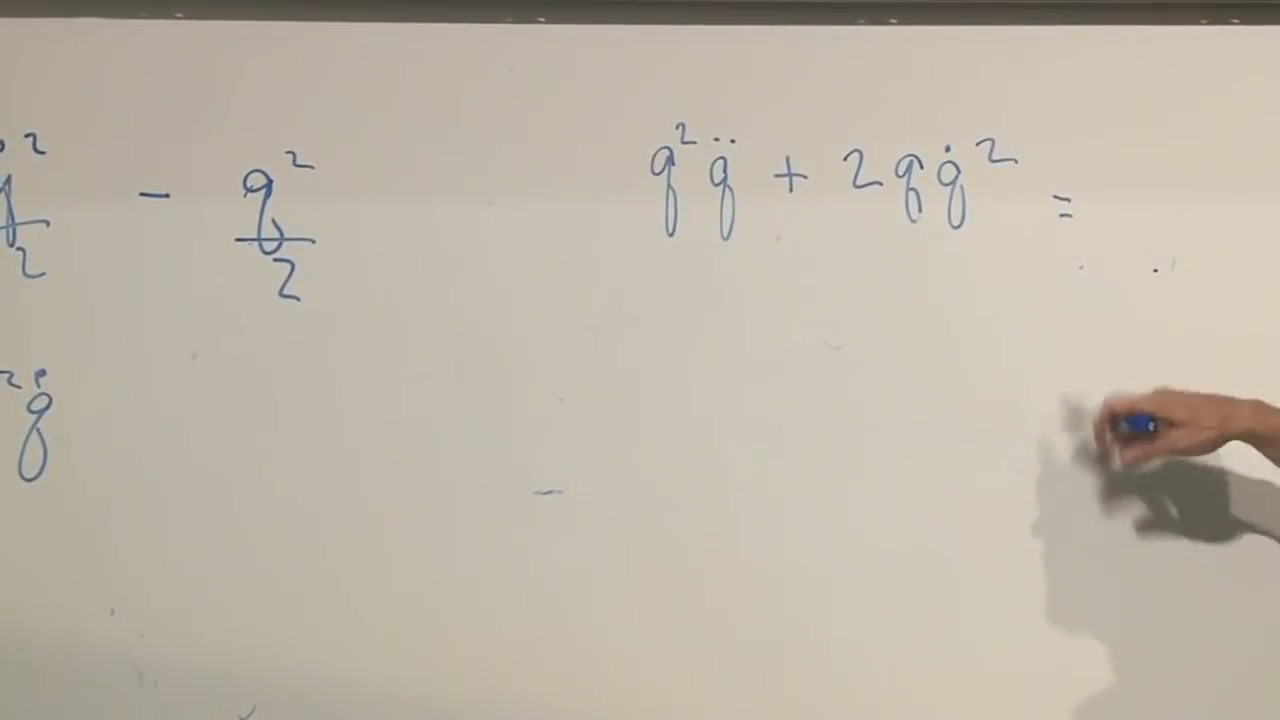
\includegraphics[width=0.80\textwidth]{lecture_05_figure_06.png}
\caption{Đạo hàm của xung lượng trong ví dụ có số hạng động năng phụ thuộc tọa độ.}
\lectureframe{01:52:32}
\end{figure}

\begin{classroomqa}
\audiencequestion{Có thể chia phương trình cho \(q\) không?
\lecturetimestamp{01:53:22--01:53:39}}
\lecturerresponse{Chỉ ở những nơi \(q\neq0\). Tại \(q=0\), hệ số động năng và ánh xạ Legendre bị suy biến, nên phép chia sẽ loại bỏ một điểm kỳ dị cần được xử lý riêng.}
\end{classroomqa}

Hamiltonian là
\begin{align}
  H&=p\dot q-L
  \notag\\
   &=q^2\dot q^2-
     \left(\frac12q^2\dot q^2-\frac12q^2\right)
  \notag\\
   &=\frac12q^2\dot q^2+\frac12q^2.
  \label{eq:l5-nonstandard-h}
\end{align}

\begin{classroomqa}
\audiencequestion{Liệu \(q^2\dot q^2/2\) vẫn có thể được gọi là động năng không?
\lecturetimestamp{01:54:41--01:55:07}}
\lecturerresponse{Có. Trong ví dụ đã giải này, Hamiltonian một lần nữa có dạng một số hạng động năng dương cộng với một số hạng thế năng. Điểm mấu chốt là các định nghĩa hình thức đã vận hành mà không cần giả định trước dạng sơ cấp với khối lượng không đổi.}
\end{classroomqa}

\section{Sự tiêu tán và nguồn gốc sâu hơn của hình thức luận}

\begin{classroomqa}
\audiencequestion{Ma sát được đưa vào một Lagrangian như thế nào?
\lecturetimestamp{01:55:09--01:56:17}}
\lecturerresponse{Không phải như một lực cơ bản trong hệ đơn giản, kín, có hữu hạn bậc tự do đang được xét ở đây. Ma sát vĩ mô là một hiệu ứng thống kê của số lượng khổng lồ các bậc tự do vi mô. Các nguyên tử ấy vẫn tuân theo cơ học cơ bản, nhưng một mô tả rút gọn không theo dõi chúng sẽ biểu lộ sự tiêu tán.}
\end{classroomqa}

\begin{classroomqa}
\audiencequestion{Hamilton đã đi đến cách phát biểu của mình như thế nào?
\lecturetimestamp{01:56:22--01:56:37}}
\lecturerresponse{Ở đây không đưa ra phép dẫn giải lịch sử nào. Nhiệm vụ quan trọng đối với học phần hiện tại là hiểu cách phát biểu ấy vận hành như thế nào.}
\end{classroomqa}

\begin{classroomqa}
\audiencequestion{Có một quy trình tổng quát hơn để thu được một Lagrangian khi nó không hiện rõ là \(T-V\) không?
\lecturetimestamp{01:56:43--01:58:54}}
\lecturerresponse{Thực nghiệm, một phỏng đoán có cơ sở, một nguyên lý đối xứng, hoặc việc dựng lại từ các phương trình mong muốn đều có thể cung cấp hàm đó. Hỏi chính phép tính ấy xem đầu vào của nó từ đâu mà có cũng giống như hỏi định nghĩa của đạo hàm rằng \(f(x)\) từ đâu mà có. Phép tính ấy cho ta biết phải làm gì một khi hàm đã được chỉ định. Vì sao các hệ kín của tự nhiên lại tuân theo cấu trúc trừu tượng này được trả lời ở mức sâu hơn bởi cơ học lượng tử.}
\end{classroomqa}

Điểm này nối với các chủ đề mở đầu của khóa học. Sự tiến hóa Hamilton cơ bản có tính tất định và khả nghịch theo nghĩa các quỹ đạo không hợp nhất và thông tin không đơn giản bị phá hủy. Mối liên hệ giữa tính chất đó và cách phát biểu không gian pha sẽ được triển khai từng bước.

\begin{classroomqa}
\audiencequestion{Liệu phép tính biến phân chỉ đơn thuần đi ngược từ các phương trình cổ điển mong muốn, và cơ học lượng tử có thu được Lagrangian của nó theo cùng cách đó không?
\lecturetimestamp{01:59:37--02:01:07}}
\lecturerresponse{Trong cách xây dựng cổ điển sơ cấp, quả thật có thể chọn một tác dụng sao cho các quỹ đạo dừng tái tạo các phương trình đã biết. Trật tự lôgic trong cơ học lượng tử thì khác: nó khởi đầu một cách tự nhiên từ Hamiltonian và có thể tiến tới một mô tả Lagrangian. Ở đó Hamiltonian trực quan hơn, mặc dù trong cơ học cổ điển ban đầu nó xuất hiện như một khái niệm trừu tượng.}
\end{classroomqa}

\begin{classroomqa}
\audiencequestion{Cơ học lượng tử có thể mô tả ma sát không?
\lecturetimestamp{02:01:08--02:02:05}}
\lecturerresponse{Có, nhưng một mô tả cơ bản phải bao gồm các bậc tự do của môi trường. Một hạt chuyển động trong một chất lỏng nhớt không thể được mô tả hoàn toàn nếu không có các hạt của chất lỏng. Ma sát là hiệu ứng tập thể phức tạp xuất hiện khi các bậc tự do đó không được theo dõi riêng lẻ.}
\end{classroomqa}